\chapter{Set-Membership Identification: Introduction}

The objective of this chapter is to introduce an approach for the parameter estimation which requires to do less strong assumption on the noise affecting the experimentally collected data. After a brief introduction with the crucial ingredients, we will go on with some instructive examples which will bring us to the complete formulation of the \textbf{Set-Membership System Identification procedure}.

\section{Ingredients for Set-Membership System Identification}
As usual in order to perform correctly the procedure of System Identification we need some crucial ingredients:
\begin{itemize}
    \itemsep-0.2em
    \item[\ding{182}] \textbf{\textsf{A-priori assumption on the system:}}
    \begin{enumerate}
        \item[\ding{51}] We use the general \textbf{regression form} 
        \begin{equation} 
            y(k)=f(y(k-1), y(k-2),  ..., y(k-n), u(k-1), ..., u(k-m), \theta)
        \end{equation}
        \item[\ding{51}] The \textbf{class of function} $\mathcal{F}$ and the order of the system $n$;     
    \end{enumerate}
   
    \item[\ding{184}] \textbf{\textsf{A-priori information of the noise}} and in particular:
    \begin{enumerate}  
        \itemsep-0.2em
        \item[\ding{51}] \textbf{Noise structure}: is referred to the way the uncertainty enters  into the problem.
        \item[\ding{51}] \textbf{Characteristic of the signal}, it is remarkable that here we assume something different and weaker. We will assume that the noise sequence/sequences (depending on the noise structure) belongs to a certain bounded set $\mathcal{B}$.
    \end{enumerate}
\end{itemize}

\section{Set-Membership Identification of LTI system with EE noise structure}
In this paragraph we will show what is obtained in term of parameter estimation, when we have that the a-priori information on the noise are the following:
\begin{itemize}
    \itemsep-0.3em
    \item[\ding{51}] The uncertainty enter in the problem as an additive term which we call $e(k)$ (the same of the first assumption of the theorem), that is:
    \begin{align*}
        y(k) = &-\theta_1{y(k-1)}-\theta_2{y(k-2)}-...-\theta_n{y(k-n)}\\
        &+\theta_{n+1}u(k)+\theta_{n+2}u(k-1)+...+\theta_{n+m+1}u(k-m) + \underbrace{e(k)}_{\textsf{EQUATION ERROR}}
    \end{align*}
    \item[\ding{51}] We suppose on the sequence characterizing the error is \textbf{bounded} (this is the crucial difference with respect to what requires the \textit{consistency theorem}), that is:
    \begin{equation}\label{eq:boundedness}
        e(k)\in\mathcal{B}_e \iff \vert e(k) \vert \le \Delta_e, \ k=1, ..., H
    \end{equation}
\end{itemize}
\subsection{Feasible Parameter Set $\mathcal{D}_\theta$}

\begin{quotation}
    \noindent
    \textsf{In this paragraph by using some examples, we will define the \textit{feasible parameter set} and its fundamental properties, in particular, it is useful to derive a \textbf{mathematical formulation of such a set} in order to explore its \textit{usefulness} and \textit{boundedness}}
\end{quotation}

\noindent
The set of solutions for the identification problem is implicitly described on what is called the \textbf{Feasible Parameter Set (FPS)}, we will indicate it with $\mathcal{D}_\theta$.

\begin{definition}[\textsf{\textbf{FEASIBLE PARAMETER SET}}] \textit{The \textbf{Feasible Parameter Set} $\mathcal{D}_\theta$ is the set of all the values of the parameter $\theta=[\theta_1 ... \theta_n]^T$ which are consistent (coherent) with all the available a-priori information (system and noise) and all the collected data (a-posteriori information).}
\end{definition}


\noindent
In order to better understand the meaning of $\mathcal{D}_\theta$ let us assume we are collecting data in the OE setup, and we know that $\vert \eta(k) \vert \le \Delta_\eta$. The input sequence, then, is perfectly known while the output is corrupted by the noise $\eta(k)$.

\begin{figure}[h]
    \centering
    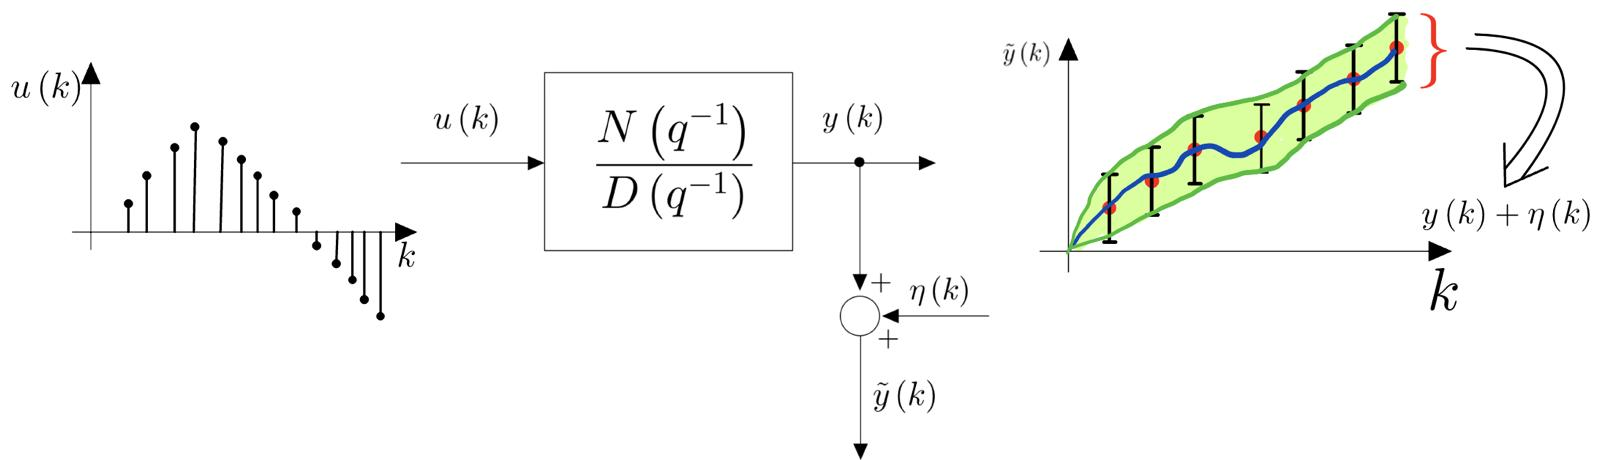
\includegraphics[scale=0.32]{img/oe_example.jpeg}
    \caption{OE set-up experiment}
\end{figure}

\noindent
The question is: \textsf{Is the SM approach providing us a pointwise estimate for the parameter $\theta$?} We will show more or less formally in the following that the answer is NO, but we can track an intuitive reasoning which will bring us to the same conclusion. \\
For this aim, given the sequence $u(k)$, we collect an output $\tilde{y}(k), \ k=0, 1, ...$. Moreover, let us suppose that for such collected data the obtained model is giving us some parameter $\theta$ such that the I/O mapping is the one indicated with the {\color{blue} blue} line. Now, since the output measurements are affected by noise, all of the samples between $[\tilde{y}(k)-\eta(k), \tilde{y}(k)+\eta(k)]$\footnote{
    See the black vertical bars
} is providing us an information which is coherent with the a-priori assumption on the noise itself. Besides, another couple of parameter $\theta_1, \theta_2$ derived from such samples, can be also the result of our identification problem. From the reasoning we have just presented we can intuitively understand that:
\begin{quotation} 
    \noindent
    \textsf{probably the parameter $\theta_i$ are provided with an \textbf{uncertainty interval} since also the experimental data are provided with uncertainty.}
\end{quotation}

\subsection{Mathematical formulation of the FPS}
We know that the system is a \textbf{second order}, \textbf{LTI one} (\textit{a-priori assumption on the system}), the uncertainty/noise enters the identification problem as additive term $e(k)$ (equation error) and it is \textbf{bounded} (that is $\vert e(k)\vert \le \Delta_e, \ k=0,1, ..., H$) (\textit{a-priori assumption on the noise}), after having collected the data $\tilde{y}(k)$, after having stimulated the system to be identified with a sequence $\tilde{u}(k)$ (\textit{a-posteriori information})\footnote{
    An EIV(Errors-in-variables) set-up is assumed, then, in order to be more precise the input is given by a subsystem, this is the reason why we have to measure it.
}, we can define the \textsf{Feasible Parameter Set} as follows:

\begin{equation} \label{eq:FPS_2nd}
    \begin{aligned}
        \mathcal{D}_\theta=&\{\theta\in\mathbb{R}^p: \ 
                \tilde{y}(k)=-\theta_1\tilde{y}(k-1)
                -\theta_2\tilde{y}(k-2)+\\
                &+\theta_3\tilde{u}(k)
                +\theta_4\tilde{u}(k-1)
                +\theta_5\tilde{u}(k-2)+e(k), \quad k=3,...,H\\
                &  \vert e(k) \vert \le \Delta_e, \quad k=1,...,H
        \}
    \end{aligned}
\end{equation}
The set (\ref{eq:FPS_2nd}) is made up of both inequality and equality constraints, moreover it appears clear that it is a \textit{subset of $\mathbb{R}^p$} with $p$ the number of parameters. There is a problem: the set $\mathcal{D}_\theta$ is defined using some inequality constraints on the noise samples $e(k)$ which are not part of the parameter space. In the following a way to eliminate such a dependence is shown, without adding any approximation or conservativeness.

\begin{equation*} 
    \begin{aligned}
        \mathcal{D}_\theta=&\{\theta\in\mathbb{R}^p: \ 
                \tilde{y}(k)+\theta_1\tilde{y}(k-1)
                +\theta_2\tilde{y}(k-2)+\\
                &-\theta_3\tilde{u}(k)
                -\theta_4\tilde{u}(k-1)
                -\theta_5\tilde{u}(k-2)=e(k), \quad k=3,...,H\\
                &  \vert e(k) \vert \le \Delta_e, \quad k=1,...,H
        \}= \\
        &\{\theta\in\mathbb{R}^p: \ 
                \vert \tilde{y}(k)+\theta_1\tilde{y}(k-1)
                +\theta_2\tilde{y}(k-2)+\\
                &-\theta_3\tilde{u}(k)
                -\theta_4\tilde{u}(k-1)
                -\theta_5\tilde{u}(k-2) \vert \le \Delta_e, \quad k=3,...,H
        \}
    \end{aligned}
\end{equation*}
In this way, we have obtained an implicit description of the \textbf{set of all the feasible solution of our identification problem} in term of a \textit{set of inequality contraints only involving $\theta$}.\\


\begin{multicols}{2}
    \noindent
    A graphical representation of such a set in a 2-dimensional parameter space is shown in the figure on the side. Here the objective is to analyze two main features of the Feasible Parameter Set by formulating the following two questions:  
    \normalsize{
    \begin{itemize}
        \itemsep-0.2em
        \item[(Q1)] \textsf{\textbf{\color{red}Boundedness}} Is this set a bounded one? Under which conditions?
        \item[(Q2)] \textsf{\textbf{\color{red}Usefulness}} What is the relation between $\mathcal{D}_\theta$ and $\theta_{\text{true}}$?
    \end{itemize}}
    \newcolumn
    \begin{center}
        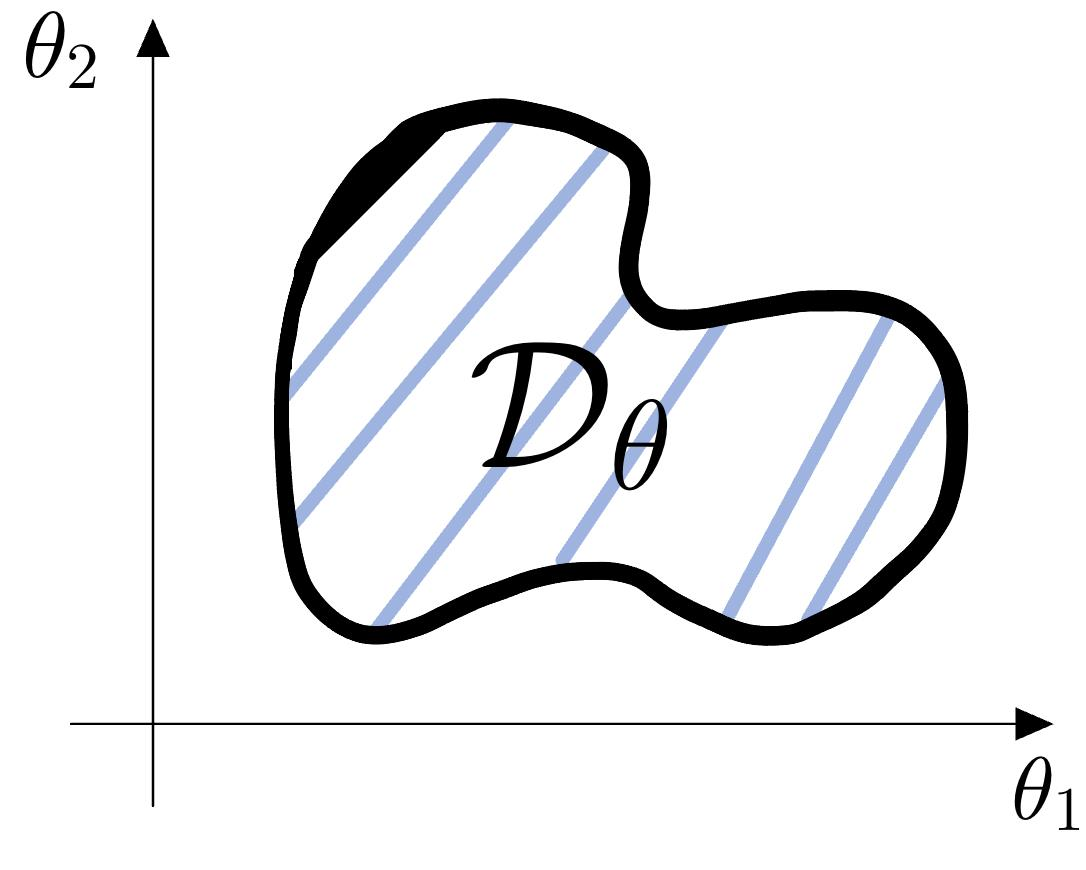
\includegraphics[scale=0.18]{img/FPS_1.jpeg}
    \end{center}
\end{multicols}
\subsubsection{Main features of $\mathcal{D}_\theta$}


\noindent
\textsf{\underline{Question Q1}} The boundedness of $\mathcal{D}_\theta$ depends on the way we collect the data (in general) ($\Rightarrow$ this concept has to be better specified in the next slides). \textit{For the moment let us assume that such a set is bounded}.\\

\noindent
\textsf{\underline{Question Q2}} Assuming that the a-priori assumptions on the system and on the noise are correct, then $\theta_{\text{true}}$ is guaranteed to belong to $\mathcal{D}_\theta$ (this is very important for further theory development).\\

\noindent
Once that we have obtained an implicit description of $\mathcal{D}_\theta$, \textit{how can we extract a useful model from it,either for simulating the system or designing a feedback controller for such a system?} Before saying it, we have to  distinguish \textit{two different classes} of SM estimation algotrithms: 
\begin{itemize}
    \itemsep-0.2em
    \item[(E1)] \textsf{\textbf{\color{red} Set-valued estimators}}, defined as estimation algorithms which provides a (possibly) conservative estimate of $\mathcal{D}_\theta$ in a \textbf{simplified geometrical form} that can be easily used to simulate or control the system; 
    \item[(E2)] \textsf{\textbf{\color{red} Pointwise Estimators}}, defined as estimation algorithms that provides a single value of $\theta$ which is an optimal estimate of $\theta_{\text{true}}$ in some sense.
\end{itemize}
Here, among all the possible estimator in the class (E1), we consider the algorithm which is providing the \textbf{minimum volume box outerbounding $\mathcal{D}_\theta$}. Such an estimator is implicitly providing what we will call \textbf{Parameter uncertainty Intervals (PUIs)}. 

\begin{multicols}{2}
    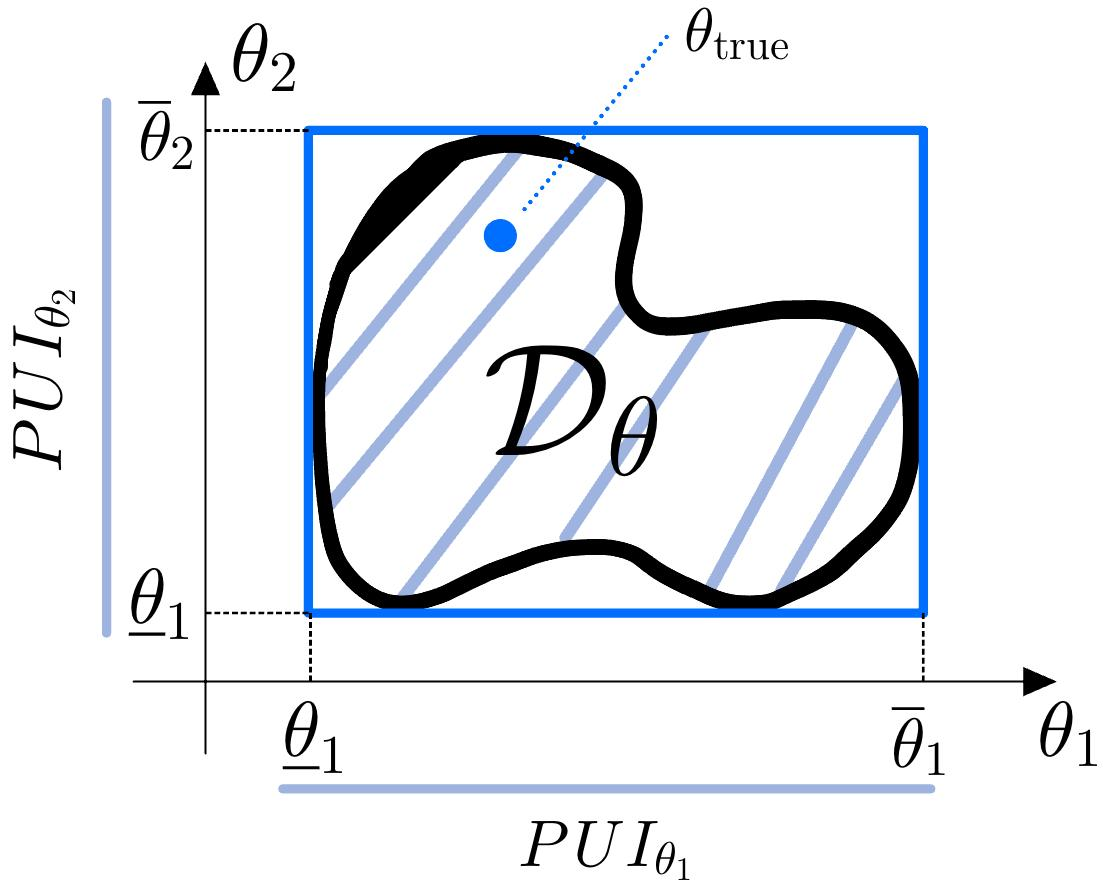
\includegraphics[scale=0.2]{img/PUI_1.jpeg}
    The PUI are defined as follows:
    \newcolumn
    \begin{equation}
        PUI_{\theta_j} = [\underline{\theta}_j,
        \overline{\theta}_j]
    \end{equation}
    where the extrema of the interval are:
    \begin{align}
        &\underline{\theta}_j \doteq \min_{\theta\in\mathcal{D}_\theta} {\theta_j}\\
        &\overline{\theta}_j \doteq \max_{\theta\in\mathcal{D}_\theta} {\theta_j} = \min_{\theta\in\mathcal{D}_\theta}{-\theta_j}
    \end{align}
    It is remarkable that each $PUI$ is providing the \textbf{minimum uncertainty interval} for each parameter $\theta_j$. In the figure are shown the $PUI$ for the feasible parameter set presented before.
\end{multicols}
\noindent 
Note the that, in the case of $\mathcal{D}_\theta \subseteq \mathbb{R}^2$ the minimum volume containing $\mathcal{D}_\theta$ is a rectangular shape whose sides are the parameter uncertainty intervals associated to $\theta_1$ and $\theta_2$.

